\documentclass{article}

\usepackage{color}
\usepackage{graphicx}
\usepackage{amsmath}
\usepackage{indentfirst}
\usepackage{float}
\usepackage{siunitx}
\begin{document}
\vspace*{0.25cm}
\hrulefill
\thispagestyle{empty}

\begin{center}
\begin{large}
\sc{UM--SJTU Joint Institute \vspace{0.3em} \\ Ve215}
\end{large}

\hrulefill

\vspace*{5cm}
\begin{Large}
\sc{{Laboratory Report}}
\end{Large}

\vspace{2em}

\begin{large}
\sc{{Exercise 5
\vspace{0.5em}

Filter Lab}}
\end{large}
\end{center}


\vfill

\begin{table}[h!]
\flushleft
\begin{tabular}{ll}
Name: Jin Minhao \hspace*{2em}&
ID: 516370910116\hspace*{2em}\\





Date: \today

\end{tabular}
\end{table}


\newpage
\section{Introduction}
\subsection{Objectives}
\begin{enumerate}
	\item  Learn about four types of filters Low-Pass, High-Pass, Band-Pass, and Band-reject.
	\item Learn about transfer functions.
	\item Predict the theoretical result and make comparison with lab data.
\end{enumerate}
\subsection{Theoretical Background}
\subsubsection{Filters}
Filters are everywhere in our lives. The circuits built to operate on signals usually
apply filters. For example, telephone lines pass the sounds at frequencies between about
100Hz and 3kHz and practically blocks all other frequencies.
\subsubsection{Transfer Function}
Mathematically, the transfer function is used to analyze what the circuit did to the
signal:
\begin{figure}[H]
	\centering
	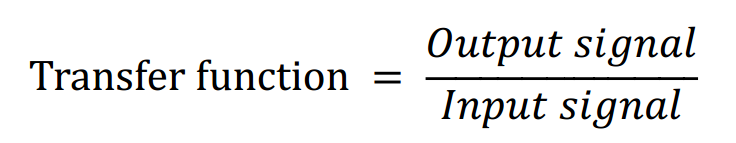
\includegraphics[width=0.4\linewidth]{D:/VE215/lab5/p1}
	\label{fig:p1}
\end{figure}
This function can also be expressed as 
\begin{figure}[H]
	\centering
	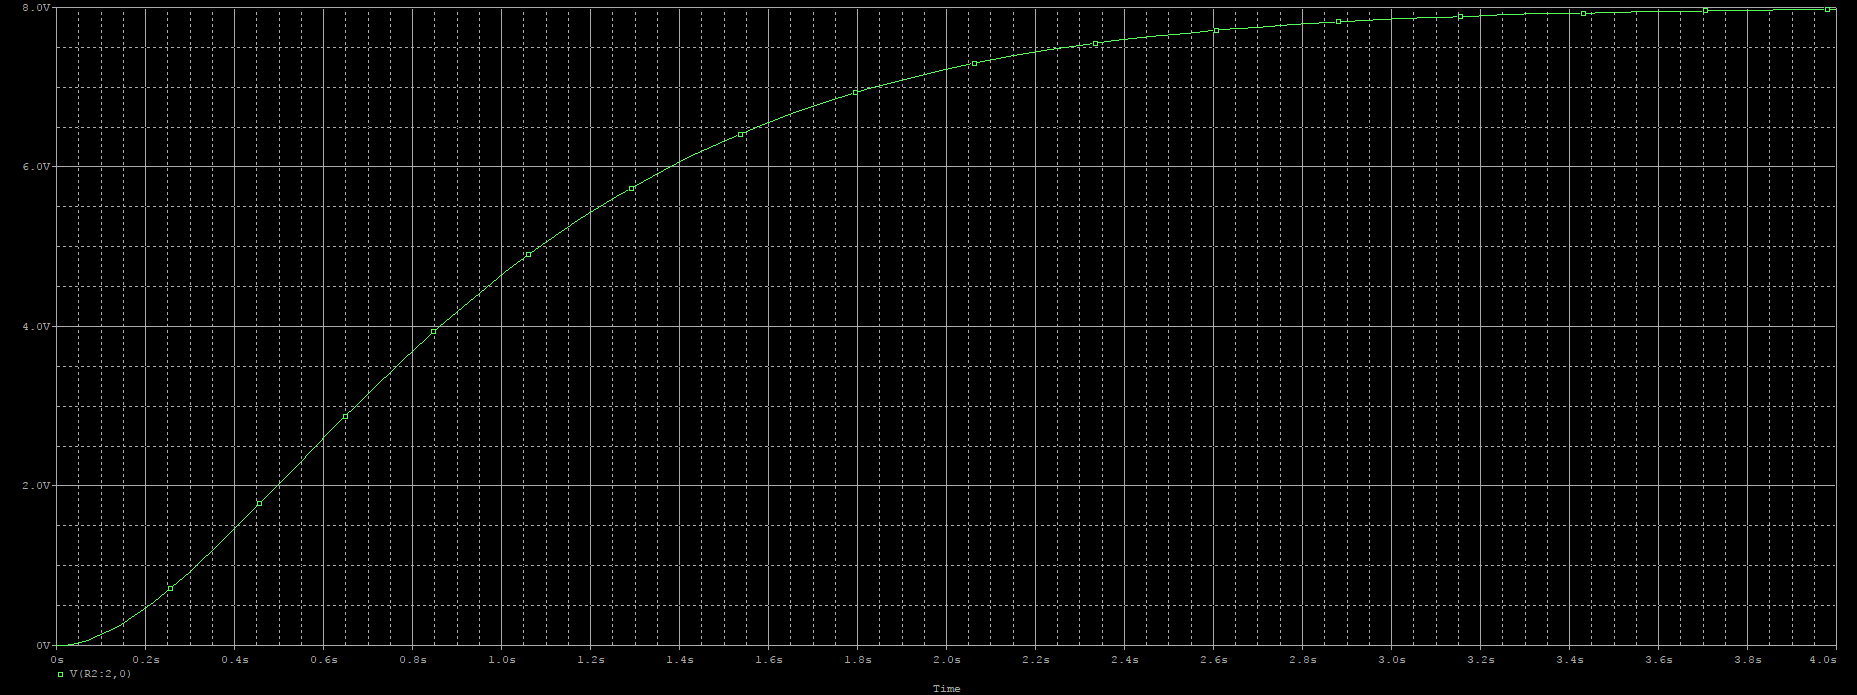
\includegraphics[width=0.2\linewidth]{D:/VE215/lab5/p2}
	\label{fig:p2}
\end{figure}
The magnitude of the transfer function is called “voltage gain”, often measured
as the ratio of the peak-to-peak (ppk) voltages:
\begin{figure}[H]
	\centering
	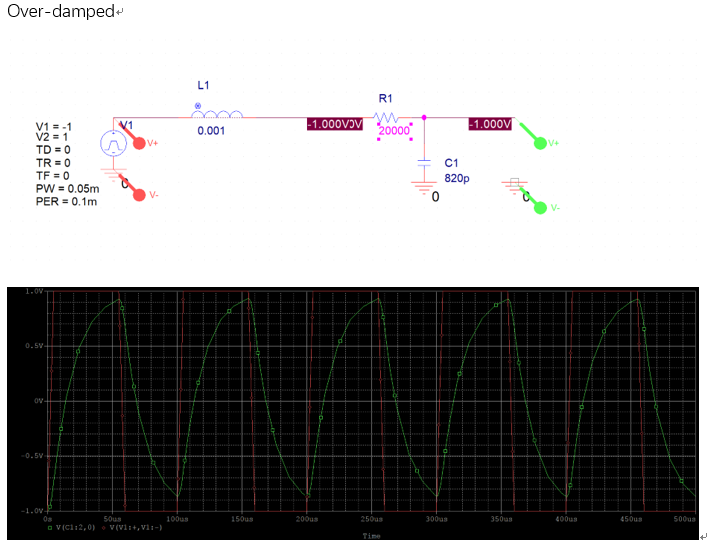
\includegraphics[width=0.3\linewidth]{D:/VE215/lab5/p3}
	\label{fig:p3}
\end{figure}
It is convenient to express and plot the magnitude of the transfer function on the
logarithmic scale using decibels:
\begin{figure}[H]
	\centering
	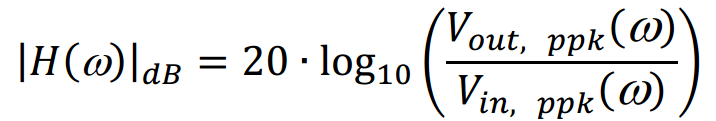
\includegraphics[width=0.3\linewidth]{D:/VE215/lab5/p4}
	\label{fig:p4}
\end{figure}
Since both ppk voltages are always positive, the transfer function magnitude is
positive and thus can always be converted to decibels. The use of decibels allows us
to review data over a broad range.
\begin{figure}[H]
	\centering
	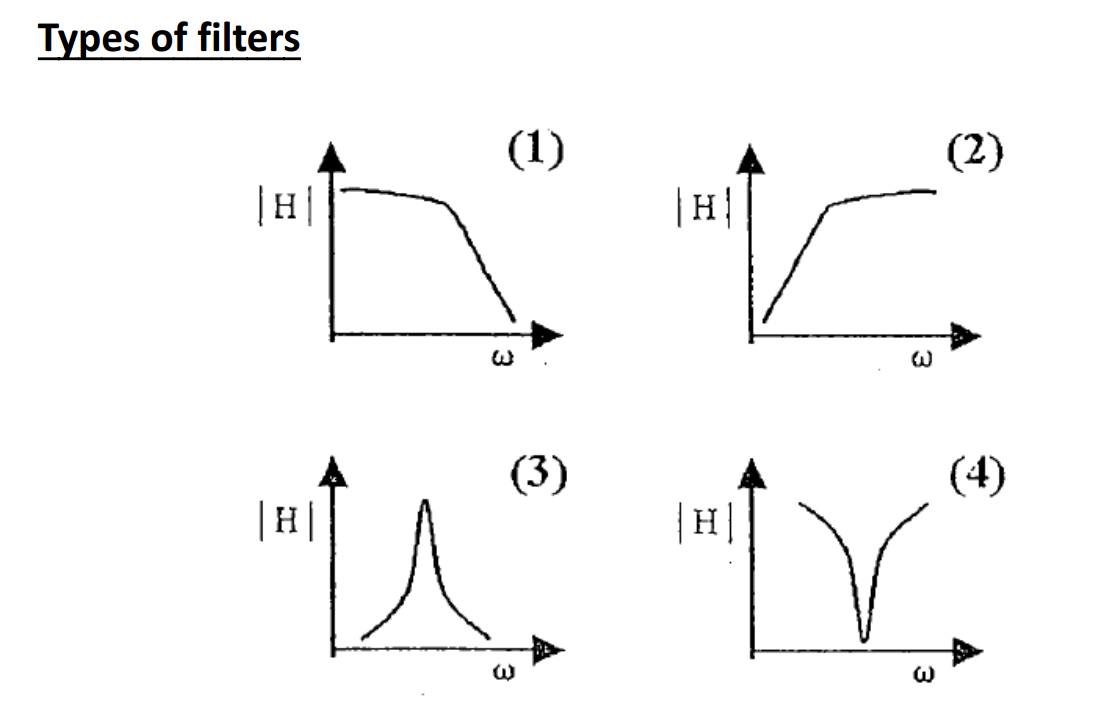
\includegraphics[width=0.7\linewidth]{D:/VE215/lab5/p5}
	\label{fig:p5}
\end{figure}
In the figure above are the four main families of filters:

(1): Low-Pass; (2): High-Pass; (3): Band-Pass; (4): Band-reject (also called
band-stop or notch)
\begin{figure}[H]
	\centering
	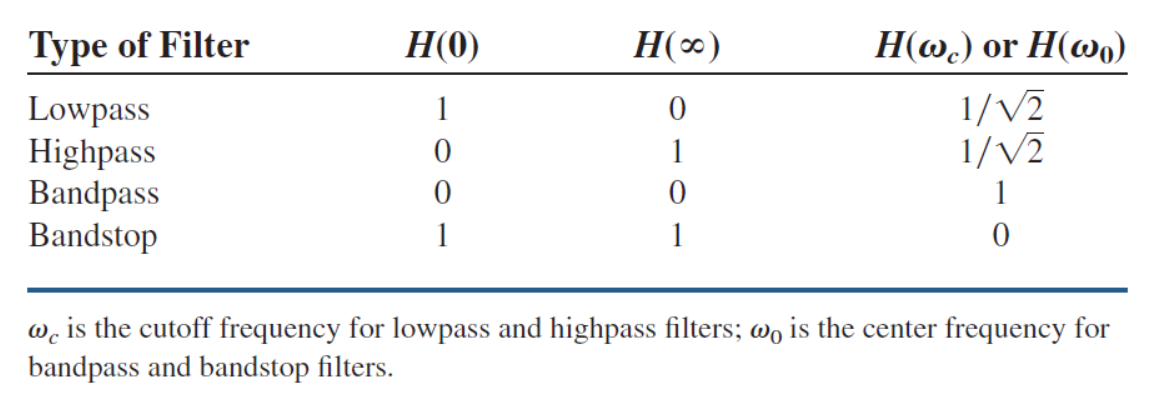
\includegraphics[width=0.7\linewidth]{D:/VE215/lab5/p6}
	\label{fig:p6}
\end{figure}
Filter circuits, which you are going to build in this lab, contain resistors,
capacitors, and inductors. They are all passive filters.
\subsubsection{High-Pass Filter}
The high-pass filter we are going to build uses a capacitor and a resistor.
\begin{figure}[H]
	\centering
	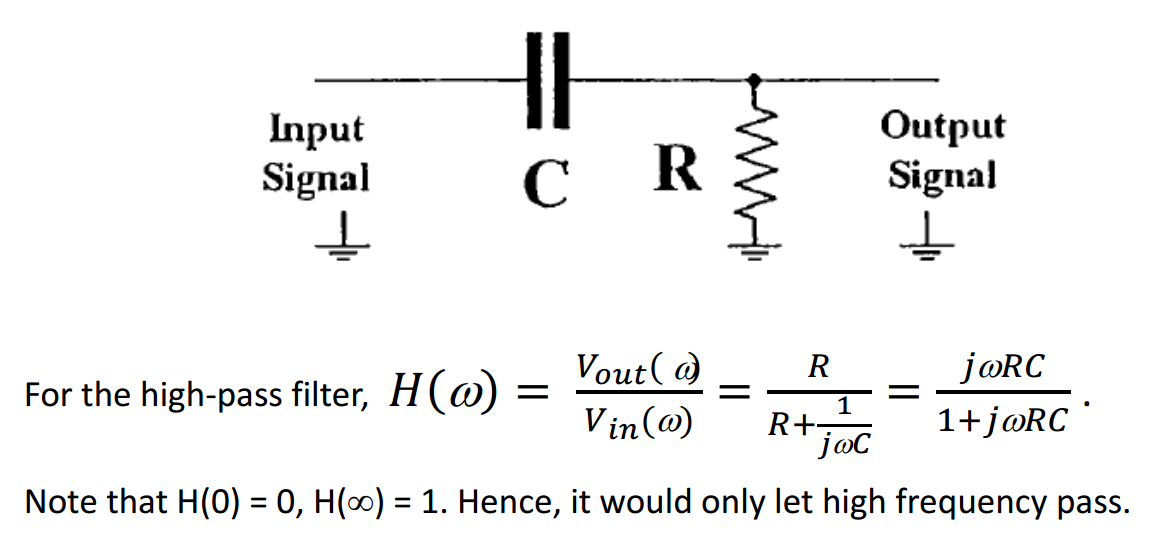
\includegraphics[width=0.7\linewidth]{D:/VE215/lab5/p7}
	\label{fig:p7}
\end{figure}
\subsubsection{Low-Pass Filter}
The low-pass filter we are going to build uses a capacitor and a resistor.
\begin{figure}[H]
	\centering
	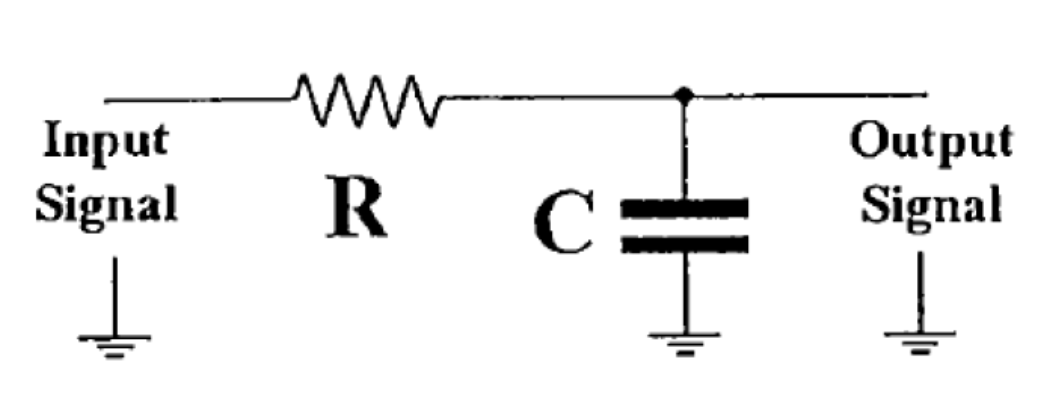
\includegraphics[width=0.7\linewidth]{D:/VE215/lab5/p8}
	\label{fig:p8}
\end{figure}
\begin{figure}[H]
	\centering
	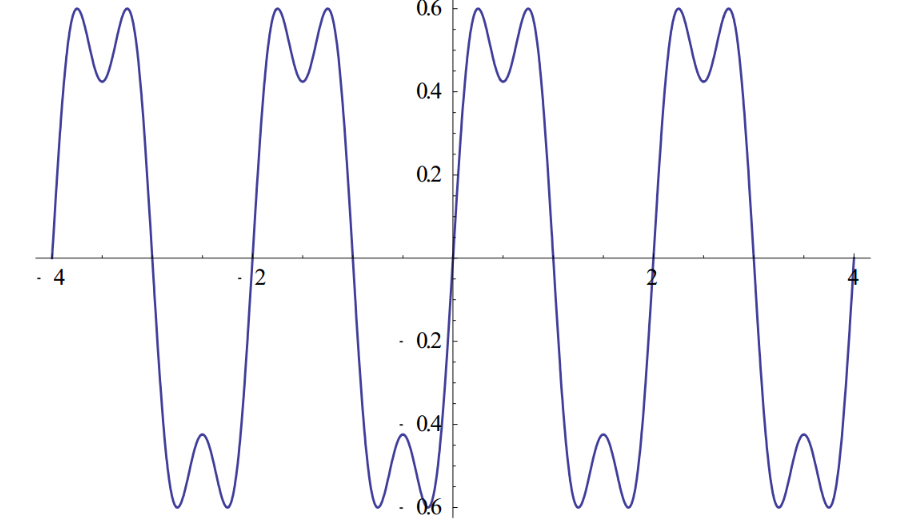
\includegraphics[width=0.7\linewidth]{D:/VE215/lab5/p9}
	\label{fig:p9}
\end{figure}
\subsubsection{Band-Pass Filter}
The band-pass filter we are going to build uses a capacitor, an inductor and a resistor.
\begin{figure}[H]
	\centering
	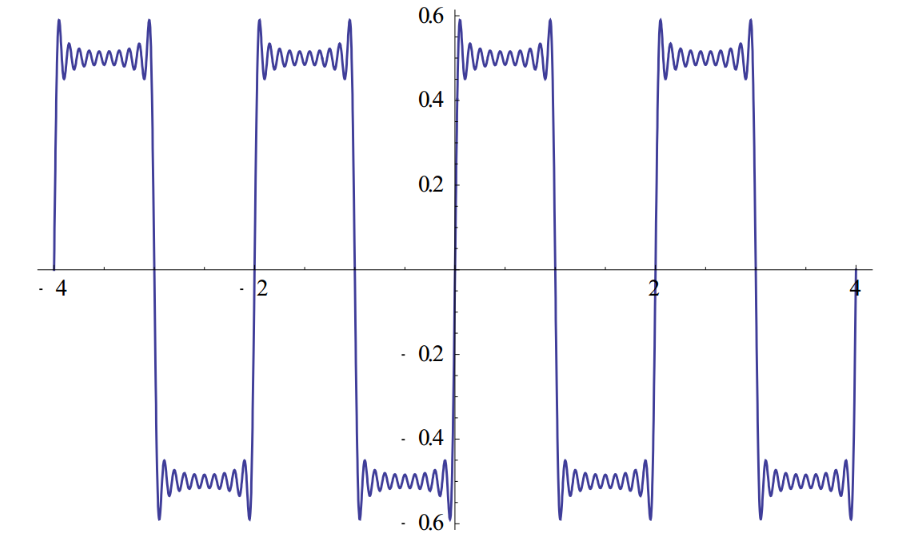
\includegraphics[width=0.7\linewidth]{D:/VE215/lab5/p10}
	\label{fig:p10}
\end{figure}
\begin{figure}[H]
	\centering
	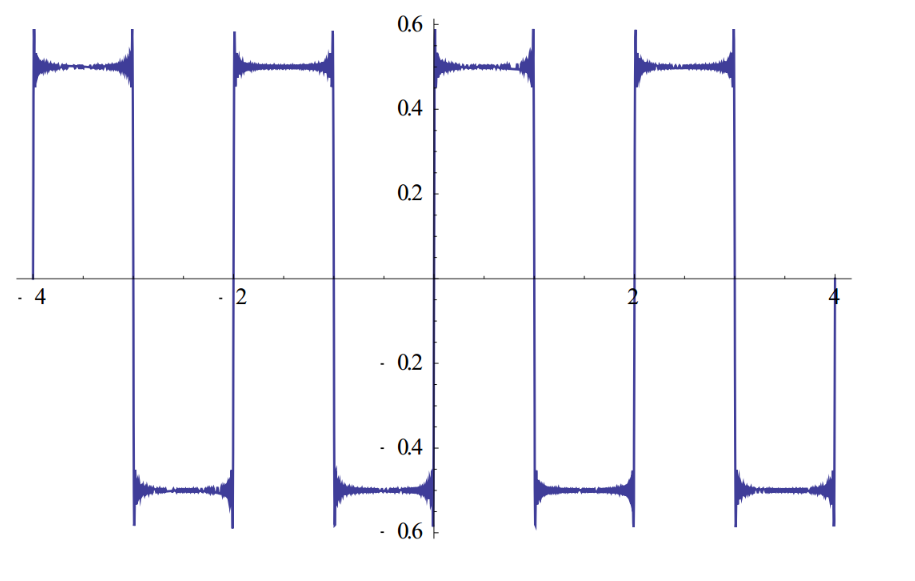
\includegraphics[width=0.7\linewidth]{D:/VE215/lab5/p11}
	\label{fig:p11}
\end{figure}
\begin{figure}[H]
	\centering
	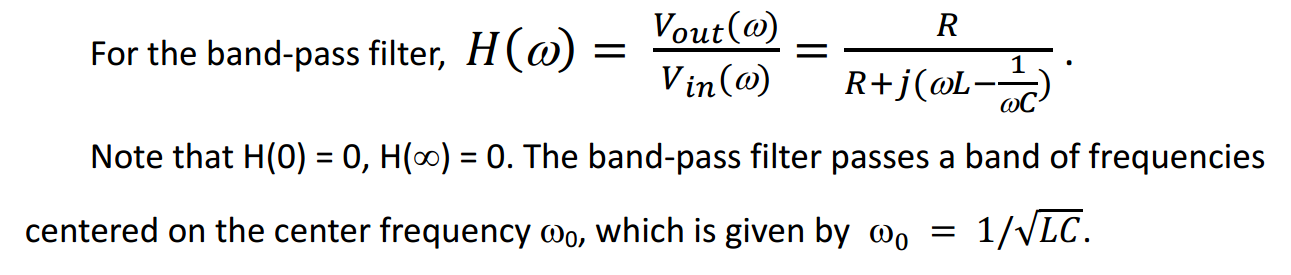
\includegraphics[width=0.7\linewidth]{D:/VE215/lab5/p12}
	\label{fig:p12}
\end{figure}
\subsubsection{Band-Stop Filter}
The band-stop filter we are going to build uses a capacitor, an inductor and a resistor.
\begin{figure}[H]
	\centering
	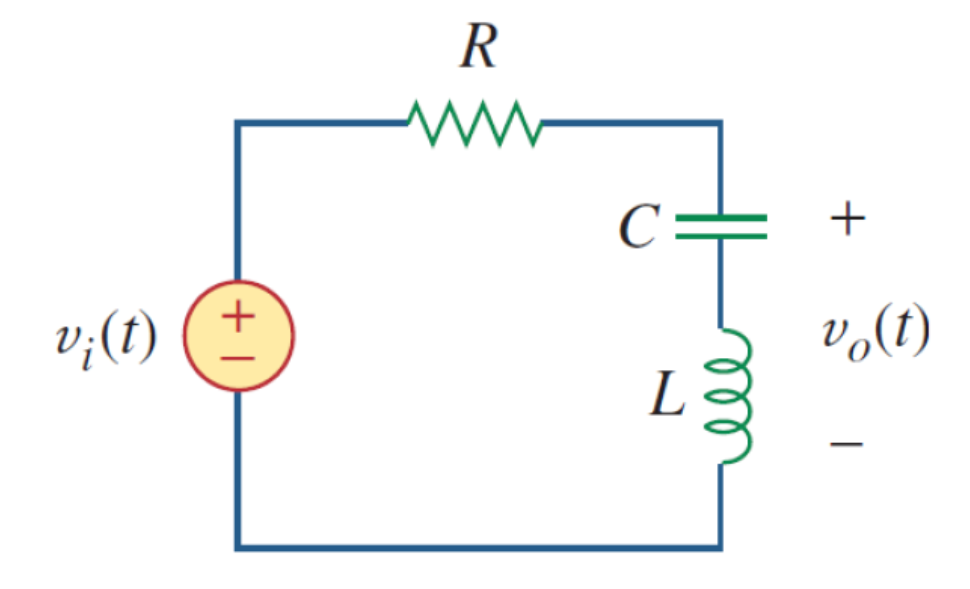
\includegraphics[width=0.7\linewidth]{D:/VE215/lab5/p13}
	\label{fig:p13}
\end{figure}
\begin{figure}[H]
	\centering
	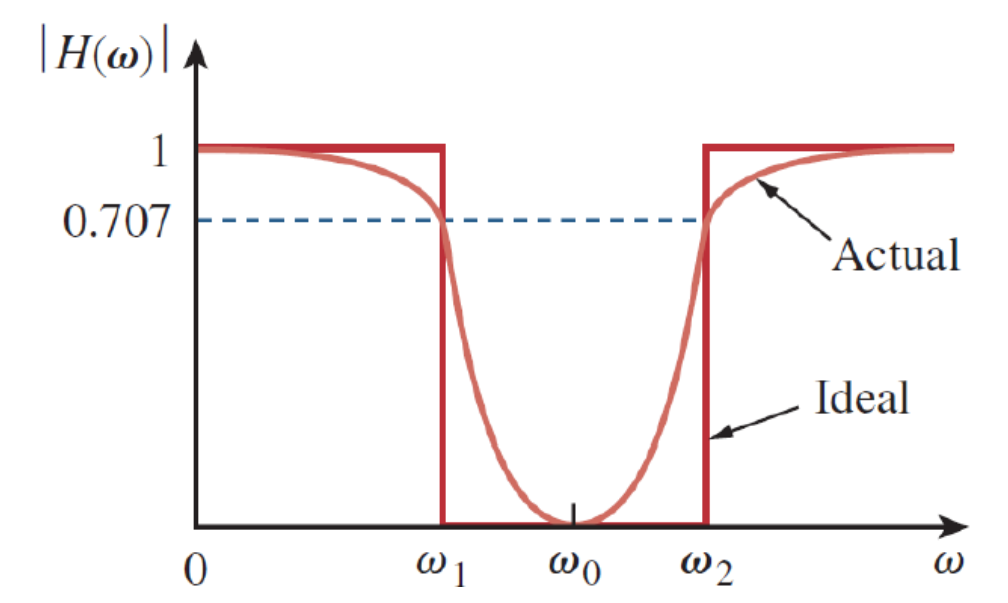
\includegraphics[width=0.7\linewidth]{D:/VE215/lab5/p14}
	\label{fig:p14}
\end{figure}
\begin{figure}[H]
	\centering
	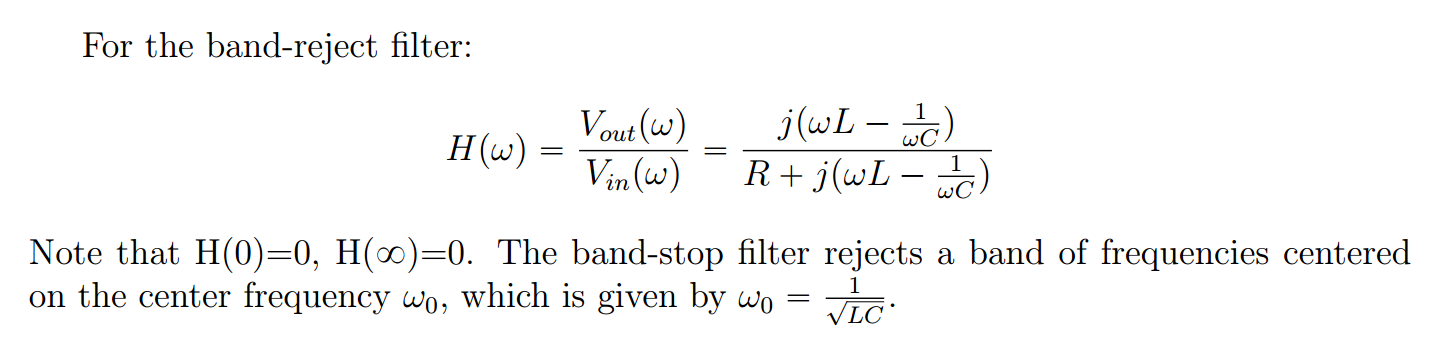
\includegraphics[width=0.7\linewidth]{D:/VE215/lab5/p15}
	\label{fig:p15}
\end{figure}
\section{Procedures}
\begin{enumerate}
	\item What is decibel value? (You may give a typical example to help your explanation.)
	What is the advantage of dB scale?
	\item How to calculate the band width of rejection of a band-reject filter? (You may
	refer to Chapter 14.7 of the textbook.)
	\item Predict the theoretical result of this lab. You need to estimate the Expected
	transfer function magnitude $|H(\omega)|$ and Expected transfer function magnitude in
	dB $|H(\omega)|_{dB}$  of all of the four types of filter. Fill in the tables in the Data Sheet
	to show the expected results (which will not be collected during the lab). Also,
	make a table for each type of filter to show the respected results (which will not
	collected during the lab as pre-lab assignment). We are using Resister of $R =
	982\Omega$; Capacitor of $C = 0.1\mu F$; Inductor of L = 1mH.
	\begin{figure}[H]
		\centering
		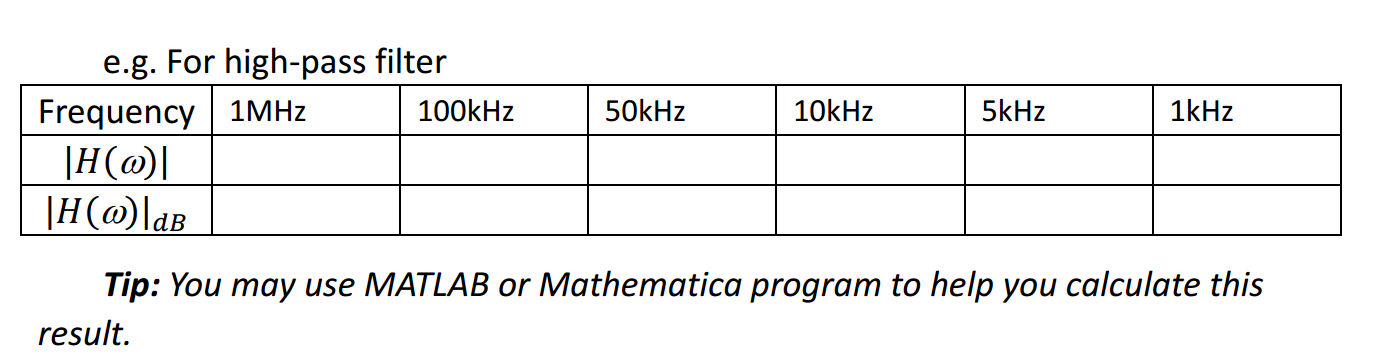
\includegraphics[width=0.7\linewidth]{D:/VE215/lab5/p16}
		\label{fig:p16}
	\end{figure}
\end{enumerate}
\section{Results}
\subsection{Low-pass Filter}
\begin{table}[H]
	\centering
\begin{tabular}{|c|c|c|c|c|c|c|}
	\hline
	Frequency & \begin{tabular}[c]{@{}c@{}}Input signal\\ amplitude\\ $V_{ppk}$\end{tabular} & \begin{tabular}[c]{@{}c@{}}Output\\ signal\\ amplitude\\ (m)$V_{ppk}$\end{tabular} & \begin{tabular}[c]{@{}c@{}}Transfer\\ function\\ generator\end{tabular} & \begin{tabular}[c]{@{}c@{}}Expected\\ transfer\\ function\\ magnitude\end{tabular} & \begin{tabular}[c]{@{}c@{}}Transfer\\ function\\ magnitude\\ in dB\end{tabular} & \begin{tabular}[c]{@{}c@{}}Expected\\ transfer\\ function\\ magnitude\\ in dB\end{tabular} \\ \hline
	1MHz      & 5.000                                                                        & 20                                                                                 & 0.0040                                                                  & 0.0016                                                                             & -47.9588                                                                        & -55.8085                                                                                   \\ \hline
	100kHz    & 5.000                                                                        & 145                                                                                & 0.0290                                                                  & 0.0162                                                                             & -30.7520                                                                        & -35.8070                                                                                   \\ \hline
	50kHz     & 5.000                                                                        & 253                                                                                & 0.0506                                                                  & 0.0324                                                                             & -25.9170                                                                        & -29.7898                                                                                   \\ \hline
	10kHz     & 5.000                                                                        & 1050                                                                               & 0.2100                                                                  & 0.1600                                                                             & -13.5556                                                                        & -15.9184                                                                                   \\ \hline
	5kHz      & 5.000                                                                        & 1950                                                                               & 0.3900                                                                  & 0.3083                                                                             & -8.1787                                                                         & -10.2191                                                                                   \\ \hline
	1kHz      & 5.000                                                                        & 4540                                                                               & 0.9080                                                                  & 0.8510                                                                             & -0.8383                                                                         & -1.4010                                                                                    \\ \hline
	500Hz     & 5.000                                                                        & 4980                                                                               & 0.9960                                                                  & 0.9556                                                                             & -0.0348                                                                         & -0.3948                                                                                    \\ \hline
\end{tabular}
\end{table}
The error and the relative error is :
\begin{table}[H]
	\centering
	\begin{tabular}{|l|l|l|l|l|}
		\hline
		Frequency & \begin{tabular}[c]{@{}l@{}}Error\\ about\\ transfer\\ function\\ amplitude\end{tabular} & \begin{tabular}[c]{@{}l@{}}Relative\\ error\\ about\\ transfer\\ function\\ amplitude\end{tabular} & \begin{tabular}[c]{@{}l@{}}Error\\ about\\ transfer\\ function\\ magnitude\\ in dB\end{tabular} & \begin{tabular}[c]{@{}l@{}}Relative\\ error\\ about\\ transfer\\ function\\ magnitude\\ in dB\end{tabular} \\ \hline
		1MHz      & 0.0024                                                                                  & $150\%$                                                                                            & 7.8497                                                                                          & $14.07\%$                                                                                                  \\ \hline
		100kHz    & 0.0128                                                                                  & $79.01\%$                                                                                          & 5.0550                                                                                          & $14.12\%$                                                                                                  \\ \hline
		50kHz     & 0.0182                                                                                  & $56.17\%$                                                                                          & 3.8728                                                                                          & $13.00\%$                                                                                                  \\ \hline
		10kHz     & 0.0500                                                                                  & $31.25\%$                                                                                          & 2.3628                                                                                          & $14.84\%$                                                                                                  \\ \hline
		5kHz      & 0.0817                                                                                  & $26.50\%$                                                                                          & 2.0404                                                                                          & $19.97\%$                                                                                                  \\ \hline
		1kHz      & 0.0570                                                                                  & $6.698\%$                                                                                          & 0.5627                                                                                          & $40.17\%$                                                                                                  \\ \hline
		500Hz     & 0.0404                                                                                  & $4.23\%$                                                                                           & 0.3600                                                                                          & $91.18\%$                                                                                                  \\ \hline
	\end{tabular}
\end{table}
\subsection{High-pass Filter}
\begin{table}[H]
	\centering
	\begin{tabular}{|l|l|l|l|l|l|l|}
		\hline
		Frequency & \begin{tabular}[c]{@{}l@{}}Input\\ signal\\ amplitude\\ Vppk\end{tabular} & \begin{tabular}[c]{@{}l@{}}Output\\ signal\\ amplitude,\\ (m)Vppk\end{tabular} & \begin{tabular}[c]{@{}l@{}}Transfer\\ function\\ magnitude\end{tabular} & \begin{tabular}[c]{@{}l@{}}Expected\\ transfer\\ function\\ magnitude\end{tabular} & \begin{tabular}[c]{@{}l@{}}Transfer\\ function\\ magnitude\\ in dB\end{tabular} & \begin{tabular}[c]{@{}l@{}}Expected\\ transfer\\ function\\ magnitude,\\ in dB\end{tabular} \\ \hline
		1MHz      & 5.00                                                                      & 4.86                                                                           & 0.9720                                                                  & 0.9999                                                                             & -0.2467                                                                         & -0.0011                                                                                     \\ \hline
		100kHz    & 5.00                                                                      & 4.86                                                                           & 0.9720                                                                  & 0.9999                                                                             & -0.2467                                                                         & -0.0724                                                                                     \\ \hline
		50kHz     & 5.00                                                                      & 4.82                                                                           & 0.9640                                                                  & 0.9995                                                                             & -0.3185                                                                         & -0.0046                                                                                     \\ \hline
		10kHz     & 5.00                                                                      & 4.70                                                                           & 0.9400                                                                  & 0.9871                                                                             & -0.5374                                                                         & -0.1126                                                                                     \\ \hline
		5kHz      & 5.00                                                                      & 4.46                                                                           & 0.8920                                                                  & 0.9513                                                                             & -0.9927                                                                         & -0.4339                                                                                     \\ \hline
		1kHz      & 5.00                                                                      & 2.25                                                                           & 0.4500                                                                  & 0.5251                                                                             & -6.9357                                                                         & -5.5952                                                                                     \\ \hline
		500Hz     & 5.00                                                                      & 1.25                                                                           & 0.2500                                                                  & 0.2948                                                                             & -12.0412                                                                        & -10.6096                                                                                    \\ \hline
		100Hz     & 5.00                                                                      & 0.285                                                                          & 0.0570                                                                  & 0.0616                                                                             & -24.8825                                                                        & -24.2107                                                                                    \\ \hline
	\end{tabular}
\end{table}
\begin{table}[H]
	\centering
	\begin{tabular}{|l|l|l|l|l|}
		\hline
		Frequency & \begin{tabular}[c]{@{}l@{}}Error\\ about\\ transfer\\ function\\ amplitude\end{tabular} & \begin{tabular}[c]{@{}l@{}}Relative\\ error\\ about\\ transfer\\ function\\ amplitude\end{tabular} & \begin{tabular}[c]{@{}l@{}}Error\\ about\\ transfer\\ function\\ amplitude\\ in dB\end{tabular} & \begin{tabular}[c]{@{}l@{}}Relative\\ error\\ about\\ transfer\\ function\\ amplitude\end{tabular} \\ \hline
		1MHz      & 0.0279                                                                                  & $2.7903\%$                                                                                         & 0.2456                                                                                          & $22300\%$                                                                                          \\ \hline
		100kHz    & 0.0279                                                                                  & $2.7903\%$                                                                                         & 0.1743                                                                                          & $240\%$                                                                                            \\ \hline
		50kHz     & 0.0355                                                                                  & $3.5518\%$                                                                                         & 0.3139                                                                                          & $682\%$                                                                                            \\ \hline
		10kHz     & 0.0471                                                                                  & $4.7716\%$                                                                                         & 0.4248                                                                                          & $377\%$                                                                                            \\ \hline
		5kHz      & 0.0593                                                                                  & $6.2336\%$                                                                                         & 0.5588                                                                                          & $129\%$                                                                                            \\ \hline
		1kHz      & 0.0751                                                                                  & $14.3020\%$                                                                                        & 6.3405                                                                                          & $107\%$                                                                                            \\ \hline
		500Hz     & 0.0448                                                                                  & $15.1967\%$                                                                                        & 1.4316                                                                                          & $13.49\%$                                                                                          \\ \hline
		100Hz     & 0.0046                                                                                  & $7.4675\%$                                                                                         & 0.6718                                                                                          & $2.77\%$                                                                                           \\ \hline
	\end{tabular}
\end{table}
\subsection{Band-pass Filter}
\begin{table}[H]
	\label{my-label}
	\begin{tabular}{|c|c|c|c|c|c|c|}
		\hline
		Frequency & \begin{tabular}[c]{@{}c@{}}Input signal\\ amplitude\\ Vppk\end{tabular} & \begin{tabular}[c]{@{}c@{}}Output\\ signal\\ amplitude\\ (m) Vppk\end{tabular} & \begin{tabular}[c]{@{}c@{}}Transfer\\ function\\ magnitude\end{tabular} & \begin{tabular}[c]{@{}c@{}}Expected\\ transfer\\ function\\ magnitude\end{tabular} & \begin{tabular}[c]{@{}c@{}}Transfer\\ function\\ magnitude\\ in dB\end{tabular} & \begin{tabular}[c]{@{}c@{}}Expected\\ transfer\\ function\\ magnitude\\ in dB\end{tabular} \\ \hline
		1MHz      & 5.00                                                                    & 193                                                                            & 0.0386                                                                  & 0.1545                                                                             & -28.2683                                                                        & -16.2240                                                                                   \\ \hline
		500kHz    & 5.00                                                                    & 1160                                                                           & 0.2320                                                                  & 0.2986                                                                             & -12.6902                                                                        & -10.4796                                                                                   \\ \hline
		100kHz    & 5.00                                                                    & 4060                                                                           & 0.8120                                                                  & 0.8485                                                                             & -1.8089                                                                         & -1.4267                                                                                    \\ \hline
		50kHz     & 5.00                                                                    & 4660                                                                           & 0.9320                                                                  & 0.9611                                                                             & -0.6117                                                                         & -0.3449                                                                                    \\ \hline
		10kHz     & 5.00                                                                    & 4780                                                                           & 0.9560                                                                  & 0.9952                                                                             & -0.3908                                                                         & -0.7261                                                                                    \\ \hline
		1kHz      & 5.00                                                                    & 2270                                                                           & 0.4540                                                                  & 0.5266                                                                             & -6.8589                                                                         & -5.5703                                                                                    \\ \hline
		500Hz     & 5.00                                                                    & 1250                                                                           & 0.2500                                                                  & 0.2921                                                                             & -12.0412                                                                        & -10.6018                                                                                   \\ \hline
	\end{tabular}
\end{table}
\begin{table}[H]
	\centering
	\begin{tabular}{|l|l|l|l|l|}
		\hline
		Frequency & \begin{tabular}[c]{@{}l@{}}Error\\ about\\ transfer\\ function\\ amplitude\end{tabular} & \begin{tabular}[c]{@{}l@{}}Relative\\ error\\ about\\ transfer\\ function\\ amplitude\end{tabular} & \begin{tabular}[c]{@{}l@{}}Error\\ about\\ transfer\\ function\\ amplitude\\ in dB\end{tabular} & \begin{tabular}[c]{@{}l@{}}Relative\\ error\\ about\\ transfer\\ function\\ amplitude\end{tabular} \\ \hline
		1MHz      & 0.1159                                                                                  & $75.01\%$                                                                                          & 12.04                                                                                           & $74.23\%$                                                                                          \\ \hline
		500kHz    & 0.0666                                                                                  & $22.30\%$                                                                                          & 2.21                                                                                            & $21.09\%$                                                                                          \\ \hline
		100kHz    & 0.0365                                                                                  & $4.30\%$                                                                                           & 0.3822                                                                                          & $26.79\%$                                                                                          \\ \hline
		50kHz     & 0.0291                                                                                  & $3.03\%$                                                                                           & 0.2668                                                                                          & $77.35\%$                                                                                          \\ \hline
		10kHz     & 0.0392                                                                                  & $3.93\%$                                                                                           & 0.3353                                                                                          & $46.17\%$                                                                                          \\ \hline
		1kHz      & 0.0726                                                                                  & $13.79\%$                                                                                          & 1.2886                                                                                          & $23.13\%$                                                                                          \\ \hline
		500Hz     & 0.0421                                                                                  & $14.41\%$                                                                                          & 1.4394                                                                                          & $13.57\%$                                                                                          \\ \hline
	\end{tabular}
\end{table}
\subsection{Band-reject Filter}
\begin{table}[H]
	\centering
	\begin{tabular}{|c|c|c|c|c|c|c|}
		\hline
		Frequency & \begin{tabular}[c]{@{}c@{}}Input signal\\ amplitude\\ Vppk\end{tabular} & \begin{tabular}[c]{@{}c@{}}Output\\ signal\\ amplitude\\ (m) Vppk\end{tabular} & \begin{tabular}[c]{@{}c@{}}Transfer\\ function\\ magnitude\end{tabular} & \begin{tabular}[c]{@{}c@{}}Expected\\ transfer\\ function\\ magnitude\end{tabular} & \begin{tabular}[c]{@{}c@{}}Transfer\\ function\\ magnitude\\ in dB\end{tabular} & \begin{tabular}[c]{@{}c@{}}Expected\\ transfer\\ function\\ magnitude\\ in dB\end{tabular} \\ \hline
		1MHz      & 5.00                                                                    & 5000                                                                           & 1                                                                       & 0.9880                                                                             & 0                                                                               & -0.1049                                                                                    \\ \hline
		500kHz    & 5.00                                                                    & 4980                                                                           & 0.5960                                                                  & 0.9544                                                                             & -4.4951                                                                         & -0.4056                                                                                    \\ \hline
		300kHz    & 5.00                                                                    & 4660                                                                           & 0.9320                                                                  & 0.8863                                                                             & -0.6117                                                                         & -1.0481                                                                                    \\ \hline
		200kHz    & 5.00                                                                    & 4140                                                                           & 0.8280                                                                  & 0.7860                                                                             & -1.6394                                                                         & -2.0911                                                                                    \\ \hline
		100kHz    & 5.00                                                                    & 2790                                                                           & 0.5580                                                                  & 0.5292                                                                             & -5.0673                                                                         & -5.5282                                                                                    \\ \hline
		50kHz     & 5.00                                                                    & 1420                                                                           & 0.2840                                                                  & 0.2763                                                                             & -10.9336                                                                        & -11.1721                                                                                   \\ \hline
		5kHz      & 5.00                                                                    & 704                                                                            & 0.1408                                                                  & 0.0976                                                                             & -17.0279                                                                        & -20.2092                                                                                   \\ \hline
		10kHz     & 5.00                                                                    & 1790                                                                           & 0.3580                                                                  & 0.2804                                                                             & -8.9223                                                                         & -11.0435                                                                                   \\ \hline
		5kHz      & 5.00                                                                    & 4540                                                                           & 0.9080                                                                  & 0.8501                                                                             & -0.8383                                                                         & -1.4105                                                                                    \\ \hline
		500Hz     & 5.00                                                                    & 4940                                                                           & 0.9980                                                                  & 0.9555                                                                             & -0.1049                                                                         & -0.3956                                                                                    \\ \hline
	\end{tabular}
\end{table}
\begin{table}[H]
	\centering
	\begin{tabular}{|l|l|l|l|l|}
		\hline
		Frequency & \begin{tabular}[c]{@{}l@{}}Error\\ about\\ transfer\\ function\\ amplitude\end{tabular} & \begin{tabular}[c]{@{}l@{}}Relative\\ error\\ about\\ transfer\\ function\\ amplitude\end{tabular} & \begin{tabular}[c]{@{}l@{}}Error\\ about\\ transfer\\ function\\ amplitude\\ in dB\end{tabular} & \begin{tabular}[c]{@{}l@{}}Relative\\ error\\ about\\ transfer\\ function\\ amplitude\end{tabular} \\ \hline
		1MHz      & 0.0120                                                                                  & $1.21\%$                                                                                           & 0.1049                                                                                          & $100\%$                                                                                            \\ \hline
		500kHz    & 0.3584                                                                                  & $37.55\%$                                                                                          & 4.0895                                                                                          & $100\%$                                                                                            \\ \hline
		300kHz    & 0.0457                                                                                  & $5.15\%$                                                                                           & 0.4364                                                                                          & $41.64\%$                                                                                          \\ \hline
		200kHz    & 0.0420                                                                                  & $5.34\%$                                                                                           & 0.4517                                                                                          & $21.60\%$                                                                                          \\ \hline
		100kHz    & 0.0288                                                                                  & $5.44\%$                                                                                           & 0.4609                                                                                          & $8.33\%$                                                                                           \\ \hline
		50kHz     & 0.0077                                                                                  & $2.78\%$                                                                                           & 0.2385                                                                                          & $2.13\%$                                                                                           \\ \hline
		10kHz     & 0.0432                                                                                  & $44.26\%$                                                                                          & 3.1813                                                                                          & $15.74\%$                                                                                          \\ \hline
		5kHz      & 0.0776                                                                                  & $27.67\%$                                                                                          & 2.1212                                                                                          & $19.20\%$                                                                                          \\ \hline
		1kHz      & 0.0579                                                                                  & $6.81\%$                                                                                           & 0.5722                                                                                          & $40.57\%$                                                                                          \\ \hline
		500Hz     & 0.0325                                                                                  & $3.40\%$                                                                                           & 0.2907                                                                                          & $73.49\%$                                                                                          \\ \hline
	\end{tabular}
\end{table}
\section{Conclusion}
Through this lab, I  learned about four types of filters Low-Pass, High-Pass, Band-Pass, and Band-reject, transfer functions
and predicted the theoretical result and make comparison with lab data.

For the low-pass filter:
\begin{figure}[H]
	\centering
	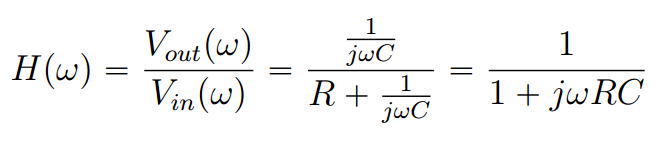
\includegraphics[width=0.3\linewidth]{pic1}
	\label{fig:pic1}
\end{figure}

For the high-pass filter:
\begin{figure}[H]
	\centering
	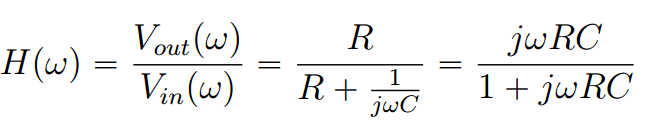
\includegraphics[width=0.3\linewidth]{pic2}
	\label{fig:pic2}
\end{figure}

For the band-pass filter:
\begin{figure}[H]
	\centering
	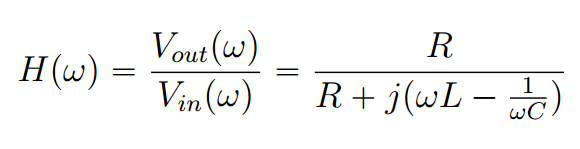
\includegraphics[width=0.3\linewidth]{pic3}
	\label{fig:pic3}
\end{figure}

For the band-reject filter:
\begin{figure}[H]
	\centering
	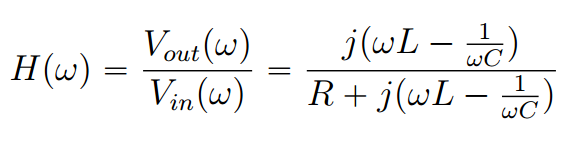
\includegraphics[width=0.3\linewidth]{pic4}
	\label{fig:pic4}
\end{figure}

These are the method to calculate the theoretical value.


It seems that some of the data is not accurate enough. The relative error is very big. I think the reason is that the function $ln$ an make an error when calculation. I find that when x is near 1, $ln x$ may have a relatively big change, and if our result has a little bit difference with the theoretical value, the result after calculation may have a huge difference. Therefore, I don't think that our experiment has some very big mistakes, but it is because the equation that results the huge error. But actually, it is still a successful experiment. Most of the data is very close to the theoretical value and their relative error is also not very big. This is a very meaningful experiment.
\end{document}